\section{Paseos, recorridos y ciclos}
\stepcounter{sec}

En la parte anterior definimos los caminos, pero dependiendo del problema, querremos modelarlo prestando atención en el movimiento dentro del grafo. Quizá nos interese fijarnos en los vértices recorridos o en los lados recorridos.

\subsection{Conexidad}
\stepcounter{subsec}

\begin{defn}
    Un \ul{paseo} $W$ es una lista $v_0, e_1, v_2, \dots, e_k, v_k$ de vértices y lados de un grafo $G$ tales que para $i = 1, \dots, k$ se tiene $f_G(e_k) = \{v_{j-1},v_j\}$. Vemos que $k$ es la cantidad de lados del paseo, y lo denotaremos por $k = \lngtd{W}$.
    
    Un \ul{recorrido} es un paseo sin lados repetidos, es decir que si $W$ es un paseo en $G$, entonces $\forall i,j$ tenemos que $i \neq j \implies e_i \neq e_j$, con $e_i, e_j \in W$.
    
    Diremos que un paseo es \ul{cerrado} si $v_0 = v_k$. También nos referiremos a la \ul{longitud} de un paseo $W$ como la cantidad de lados que tiene el paseo y lo denotaremos con $\lngtd{W}$.
\end{defn}

Es inmediato suponer que existe una relación entre los paseos y los caminos (que definimos en la sección anterior). Veamos concretamente cómo se relacionan:

\begin{lem}
    Todo paseo de $u$ a $v$ contiene un camino de $u$ a $v$.
\end{lem}

\begin{proof}
    Pasaremos a realizar la demostración de este lema por inducción: Sea $W$ un camino con $\lngtd{W} = n$. Si $n = 0$, entonces el paseo no tiene lados, por lo tanto $W$ consiste de un único vértice y $u = v$. De esta forma $W$ contiene un camino de $u$ a $v$ de longitud $0$.
    
    \begin{marginfigure}
        \centering
        \begin{tikzpicture}
            \SetGraphUnit{1}
            \Vertex{u}
            \WE(u){v1}
            \WE(v1){v2}
            \WE(v2){v3}
            \WE(v3){w}
            \SO(w){v}
            \Edges(u,v1,v2,v3,w,v)
            \Loop[dist=1cm](w)
        \end{tikzpicture}
        \caption{Situación descrita en la demostración del lema. El bucle en $w$ representa los vértices entre $w$ y su repetición. Al igual que ocurre en $w$, esta situación se puede generalizar para cualquier vértice.}
    \end{marginfigure}
    
    Supongamos ahora que el teorema se cumple para $n < k$. Toca demostrar para $n = k$: Si $W$ no tiene vértices repetidos, entonces todos sus vértices y lados forman un camino de $u$ a $v$. Si $W$ tiene un vértice repetido $w$, entonces omitamos todos los lados y vértices que aparecen entre $w$ y su repetición, de esta forma obtenemos un paseo $W'$ contenido en $W$. Como $\lngtd{W'} < k$, podemos aplicar la H.I y hay un camino $P$ de $u$ a $V$ contenido en $W'$. Ya que $W' \subset W$, entonces el camino $P$ está contenido en $W$.
    
    De esta forma, hemos demostrado el lema por inducción.
\end{proof}

\begin{defn}
    Sean $G$ un grafo y $u, v \in V(G)$. Diremos que $u$ está \ul{conectado} con $v$ si existe un camino de $u$ a $v$ (y de lo contrario, \ul{desconectado}). La \ul{relación de conexidad} sobre $V(G)$ consiste en los pares ordenados $(u,v)$ tales que $u$ está conectado a $v$. Las clases de equivalencia de esta relación son las componentes del grafo $G$, es decir todo subgrafo de $G$ tal que es conexo maximal.
\end{defn}

\begin{ejem}\label{ejem:cortes}
    El grafo de abajo tiene $4$ componentes, una de ellas siendo un vértice aislado. Los conjuntos de vértices de cada componente son $\{a,b\}$, $\{c,d,e,f,g\}$, $\{h\}$ e $\{i,j,k\}$, y estas son las clases de equivalencia respecto a la relación de conexidad.
    
    \begin{figure}
        \centering
        \begin{tikzpicture}
            \SetGraphUnit{1}
            \Vertex{a}
            \SO(a){b}
            \Edges(a,b)
            \Vertex[x=1 , y=0]{c}
            \EA(c){d}
            \SO(d){g}
            \EA(d){e}
            \EA(e){f}
            \Edges(c,g,d,c,d,e,g,e,f)
            \Vertex[x=3.5 , y=-1]{h}
            \Vertex[x=5 , y=-1]{i}
            \Vertex[x=5.5 , y=0]{j}
            \EA(j){k}
            \Edges(i,j,k)
        \end{tikzpicture}
        \caption{Grafo con $4$ componentes.}
    \end{figure}
\end{ejem}

Vemos del ejemplo anterior que eliminar un vértice o lado puede incrementar el número de componentes. Por ejemplo, si eliminamos el lado que incide en $i$ pasamos a tener $5$ componentes, lo mismo ocurre si eliminamos $j$ y los lados que inciden con él.

\begin{defn}
    Un \ul{lado-corte} ó \ul{vértice-corte} de un grafo es un lado o vértice que al retirarlo del grafo incrementa el número de componentes. Escribimos $G - e$ o $G - M$ para denotar al subgrafo de $G$ obtenido al retirar el lado $e$ o el conjunto de lados $M$. Escribimos $G - v$ ó $G - S$ para denotar al subgrafo obtenido al retirar el vértice $v$ o el conjunto de vértices $S$.
\end{defn}

Es importante resaltar que las componentes son disjuntas dos a dos, es decir que no existe un par de componentes que comparta un vértice. Añadir un lado que une a dos vértices en componentes distintas hace que se reduzca en $1$ el número de componentes. De esta forma, añadir un lado reduce el número de componentes en $0$ o en $1$, y eliminar un lado incrementa el número de componentes por $0$ o $1$.

\begin{pro}\label{pro:componentes}
    Todo grafo con $n$ vértices y $k$ lados tiene al menos $n-k$ componentes.
\end{pro}

\begin{proof}
    Un grafo con $n$ vértices sin lados tiene $n$ componentes. Sabemos por la discusión anterior que cada lado reduce el número en componentes en máximo $1$, así que cuando se han añadido $k$ lados, el número de componentes sigue siendo mayor o igual a $n-k$.
\end{proof}

\begin{ejem}
    Para el grafo presentado en el ejemplo \ref{ejem:cortes}, tenemos que
    
    \begin{itemize}
        \item Lados-corte: $ab$, $ef$, $ij$, $jk$.
        \item Vértices-corte: $e$, $j$.
    \end{itemize}
\end{ejem}

\begin{defn}
    Sean $G$ un grafo y $T \subseteq V(G)$. El \ul{grafo inducido} denotado por $G[T]$ está conformado por $T$, $f_{G|T}$ y todo lado $e \in E(G)$ que cumpla lo siguiente: para algún par no ordenado $\{u,v\}$ con $u,v \in V(T)$, se tiene que $\{u,v\} = f_G(e)$. Es decir, que el grafo inducido consiste también de todos los lados de $G$ cuyos vértices están contenidos en $V(T)$.
\end{defn}

Para esta definición, es importante resaltar que un conjunto de vértices $S$ es un conjunto independiente sii el grafo inducido por $S$ no tiene lados.

\begin{ejem}
    Nuevamente, en el grafo del ejemplo \ref{ejem:cortes}, tenemos que $C_4$ y $P_5$ son subgrafos \textbf{NO} inducidos, y $P_4$ es un subgrafo inducido: Puede ser inducido por $\{c,g,e,f\}$ o por $\{c,d,e,f\}$.
\end{ejem}

\begin{teo}
    Sean $G$ un grafo y $e \in E(G)$, entonces $e$ es un lado-corte sii no pertenece a un ciclo.
\end{teo}

\begin{proof}
    Sea $e$ un lado de un grafo $G$ (con vértices $x,y$) y sea $H$ la componente que contiene a $e$. Como al eliminar $e$ ninguna otra componente se ve afectada, es suficiente probar que $H - e$ es conexo si y sólo si $e$ pertenece a un ciclo. Probemos ambas implicaciones:
    
    \begin{enumerate}
        \item[$\Leftarrow$] Supongamos que $e$ pertenece a un ciclo $C$ de $H$. Escojamos $u, v \in V(H)$. Como $H$ es conexo, entonces $H$ tiene un camino $P$ de $u$ a $v$. Si $P$ no contiene a $e$, entonces $P$ está en $H - e$, como esto es para todo $u, v \in V(H)$, $H - e$ es conexo. Si $P$ contiene a $e$ supongamos en primer lugar y sin pérdida de generalidad que $x$ está entre $u$ e $y$ en $P$. Como $H - e$ contiene un camino de $u$ a $x$ (el cual está en $P$), un camino de $x$ a $y$ (está en $C$) y un camino de $y$ a $v$ (está en $P$ nuevamente), por la transitividad de la relación de conexidad tenemos que eso implica que $H - e$ tiene un camino de $u$ a $v$, y esto se cumple para todo $u, v \in V(G)$.
        
        De esta forma, $u, v \in V(H)$ y $H - e$ es conexo.
        
        \item[$\Rightarrow$] Supongamos ahora que $H - e$ es conexo. Esto implica que existe un camino de $x$ a $y$, y si se agrega nuevamente el lado $e$, se tiene un ciclo. Por lo tanto $e$ pertenece a un ciclo.
    \end{enumerate}
    
    De esta manera queda demostrado.
\end{proof}

\subsection{Ciclos y grafos bipartitos}
\stepcounter{subsec}

Ahora estudiaremos la relación entre ciclos impares y grafos bipartitos:

\begin{lem}
    Todo paseo cerrado impar contiene un ciclo impar.
\end{lem}

\begin{proof}
    Pasaremos a hacer esta esta demostración por inducción. Sea el camino $W$ con $\lngtd{W} = l$. Si $l = 1$ entonces $W$ contiene un camino cerrado de longitud $1$, es decir un ciclo formado únicamente por un bucle, y queda demostrado el caso base.
    
    Asumamos que el teorema se cumple para $l < n$. Supongamos ahora $l = n$. Si $W$ no repite vértices excepto los extremos entonces el paso describe un ciclo y queda demostrado. Supongamos que $W$ repite vértices y sea $v$ el primer vértice repetido en $W$. Entonces $W$ consta de dos partes: un paseo cerrado par y un paseo cerrado impar. Luego podemos aplicar hipótesis inductiva en el paseo cerrado impar, y tenemos que este paseo contiene un ciclo impar. Como este ciclo está contenido en $W$, entonces $W$ contiene un ciclo impar.
    
    \begin{figure}
        \centering
        \begin{tikzpicture}[scale=0.7]
            \SetGraphUnit{2}
            \GraphInit[vstyle=Classic]
            \SetVertexNoLabel
            \Vertex{1}
            \Vertex[x=1, y=0]{2}
            \Vertex[x=1, y=2]{3}
            \Vertex[x=2, y=0]{4}
            \Vertex[x=2, y=2]{5} 
            \Vertex[x=3, y=0]{6}
            \Vertex[x=3, y=2]{7}
            \Vertex[x=4, y=1]{8}
            \Vertex[x=5, y=0]{9}
            \Vertex[x=5, y=2]{10}
            \Vertex[x=6, y=1]{11}
            \Vertex[x=7, y=0]{12}
            \Vertex[x=7, y=2]{13}
            \Vertex[x=8, y=1]{14}
            \node[yshift=-0.4cm] at (4,1) {$v$};
            \Edges(1,2,5,3,1)
            \Edges(5,4,6,8,7,5)
            \Edges(8,9,11,10,8)
            \Edges(11,12,14,13,11)
        \end{tikzpicture}
        \caption{Ejemplo de la situación descrita en el teorema. Vemos que a partir de $v$ podemos obtener $2$ caminos donde uno tiene un ciclo impar.}
    \end{figure}
\end{proof}

\begin{teo}[Teorema de König]\label{teo:konig}
    Un grafo es bipartito sii no tiene ciclos impares.
\end{teo}

\begin{proof}
    Pasemos a demostrar cada sentido:
    
    \begin{enumerate}
        \item[$\Rightarrow$] Sea $G$ un grafo bipartito. Entonces todo camino es alternante entre cada parte de $G$, por lo tanto si se parte de un conjunto independiente, para retornar a él necesitaremos agregar una cantidad par de lados a la partición. Por lo tanto no hay ciclos impares en $G$.
        
        \item[$\Leftarrow$] Supongamos ahora que $G$ no tiene ciclos impares. Para el análisis que realizaremos, basta tomar en cuenta las componentes de $G$ no-triviales. Sean $H$ una componente no trivial de $G$ y $u \in V(H)$. Para cada $x \in V(H)$ definamos $f(x)$ como la mínima longitud de un camino de $u$ a $x$. Definimos también
        
        \[
        A = \{x \in V(H) : \text{$f(x)$ es par}\} \quad \text{y} \quad B = V(H) - A
        \]
        
        Entonces $V(H) = A \cup B$. Sea ahora un lado $e \in E(H)$ incidente en los vértices $x, y$. Elegimos caminos de longitud mínima de $x$ a $u$ y de $y$ a $u$. Si ambos $x$ e $y$ están en $A$ ó $B$, entonces la suma de la longitud de ambos caminos es par, si agregamos el lado $e$, la suma es impar. Por lo tanto, tenemos un paseo cerrado impar y por el teorema anterior, este paseo contiene un ciclo impar, lo cual es una contradicción ya que $G$ no contiene ciclos impares. Por lo tanto $A$ e $Y$ son conjuntos independientes y $H$ es bipartito.

        \begin{figure}
            \centering
            \begin{tikzpicture}
                \SetGraphUnit{2}
                \GraphInit[vstyle=Classic]
                \SetVertexNoLabel
                \Vertex{u}
                \EA(u){1}
                \EA(1){2}
                \Vertex[x=7, y=-1]{x}
                \Vertex[x=7, y=1]{y}
                \node[xshift=-0.4cm] at (0,0) {$u$};
                \node[xshift=0.4cm] at (7,-1) {$x$};
                \node[xshift=0.4cm] at (7,1) {$y$};
                \Edges(u,1,2)
                \Edge(x)(y)
                \tikzset{EdgeStyle/.append style = {bend right}}
                \Edge(2)(x)
                \tikzset{EdgeStyle/.append style = {bend left}}
                \Edge(2)(y)
            \end{tikzpicture}
        \end{figure}
    \end{enumerate}
\end{proof}

\begin{prob}\label{prob:aerolineas}
    Un sistema de tráfico aéreo con $k$ aerolíneas presta servicio de ida y vuelta entre ciudades con la condición de que por ninguna aerolínea se puede hacer un recorrido cíclico impar. ¿Cuál es la máxima cantidad de ciudades que puede atender el sistema?
    
    \begin{marginfigure}
        \centering
        \begin{tikzpicture}
            \GraphInit[vstyle=Classic]
            \SetVertexNoLabel
            \grComplete[RA=2]{6}
            \end{tikzpicture}
        \caption{Cada vértice representa a una aerolínea.}
        \label{fig:aerolineas}
    \end{marginfigure}
    
    Vemos que al modelar este problema se presentan las siguientes características:
    
    \begin{enumerate}
        \item Para cada aerolínea tenemos un subgrafo del grafo completo $K_n$ si son $n$ ciudades.
        \item Entonces $K_n = G_1 \cup \dots \cup G_n$.
    \end{enumerate}
    
    Lo que queremos en este problema es contestar lo siguiente: ¿cuál es el máximo $n$ tal que $K_n$ es unión de $k$ subgrafos cada uno de los cuales no tiene ciclos impares? Por el teorema de König, queremos hallar el máximo $n$ tal que $K_n$ es unión de $k$ subgrafos bipartitos.
    
    Para resolver este problema, codifiquemos los vértices de $K_n$ con $k$-tuplas binarias: Para cada $j \in \{1, \dots, k\}$ definimos
    
    \[
    A_j = \{v \in V(K_n) : v_j = 1\} \quad \text{y} \quad B_j = V(K_n) - A_j
    \]
    
    Luego $G_j$ es el grafo bipartito con bipartición $\{A_j, B_j\}$ y $v$ es adyacente a $w$ si y sólo si $v_j \neq w_j$. Como teníamos que $G = G_1 \cup \dots \cup G_k$ entonces el máximo $n$ es $2^k$.
\end{prob}

De esta forma, hemos demostrado también el siguiente resultado:

\begin{teo}
    El grafo completo $K_n$ puede ser escrito como la unión de $k$ grafos bipartitos sii $n \leq 2^k$.
\end{teo}

\subsection{Circuitos eulerianos}
\stepcounter{subsec}

Para esta sección, regresaremos al análisis de \nameref{prob:konisberg}. Lo que los ciudadanos de Kónisberg querían conseguir era un recorrido cerrado que contenga todos los vértices del grafo \ref{fig:konisberg-model}. Como hemos observado antes, una condición necesaria para la existencia de dicho recorrido es que todos los vértices deben ser de grado par y pertenecer a la misma componente del grafo.

En 1736 Euler estableció que esta condición es también suficiente. Más adelante Heierholzer en 1873 publicó la primera demostración completa. En honor a Euler tenemos la siguiente definición:

\begin{defn}
    Un grafo $G$ es \ul{euleriano} si tiene un recorrido cerrado que contiene todos los lados de $G$. Llameremos \ul{circuito} a un recorrido cerrado (no repetimos el punto inicial sino que hacemos uso de la notación cíclica). Un circuito de $G$ es \ul{euleriano} si contiene todos los lados de $G$.
    
    Un vértice de un grafo es \ul{par (o impar)} si tiene grado par (o impar). Un grafo es \ul{par} si todos sus vértices son pares. El grado de un vértice en un grafo con bucles se define igual que antes y cada bucle en dicho vértice contribuye en $2$. Así no se altera la paridad del grafo ni la existencia de circuitos eulerianos (excepto si se trata de un bucle en una componente trivial).
\end{defn}

Veamos el siguiente lema:

\begin{lem}\label{lem:2.3.1}
    Si todo vértice de un grafo (finito) $G$ tiene grado al menos $2$, entonces $G$ contiene un ciclo.
\end{lem}

\begin{proof}
    Si $G$ tiene bucles, entonces ese bucle es un $1$-ciclo. Supongamos entonces que $G$ no tiene ciclos. Consideremos un camino maximal $P$ en $G$ (esto podemos hacerlo porque $G$ es finito). Si $v$ es un extremo de $P$, por maximalidad de $P$ y por hipótesis, $v$ tiene al menos dos vecinos en $P$. Como resultado, tenemos ciclo en $G$ y queda demostrado.
    
    \begin{figure}
        \centering
        \begin{tikzpicture}
            \SetGraphUnit{2}
            \GraphInit[vstyle=Classic]
            \SetVertexNoLabel
            \Vertex{u}
            \EA(u){1}
            \EA(1){2}
            \EA(2){3}
            \EA(3){v}
            \EA(v){4}
            \node[yshift=-0.4cm] at (0,0) {$u$};
            \node[yshift=-0.4cm] at (8,0) {$v$};
            \Edges(u,2,3,v,4)
            \tikzset{EdgeStyle/.append style = {bend right}}
            \Edge(u)(2)
            \tikzset{EdgeStyle/.append style = {bend left}}
            \Edge(u)(v)
        \end{tikzpicture}
    \end{figure}
\end{proof}

Ahora pasaremos a demostrar como tal el resultado mencionado al principio de esta sección:

\begin{teo}\label{teo:suf-euler}
    Un grafo $G$ es euleriano sii $G$ es par y tiene a lo sumo una componente no-trivial.
\end{teo}

\begin{proof}
    Demostremos ambas implicaciones:
    
    \begin{enumerate}
        \item[$\Leftarrow$] Supongamos que $G$ es un grafo par que contiene a lo sumo una componente no-trivial. Realizaremos esta prueba por inducción sobre el número de lados. Sea entonces $m = |E(G)|$. Si $m = 0$ entonces tenemos que $G$ está formado únicamente por un vértice aislado y el circuito buscado es el conformado por ese vértice solamente.
        
        Supongamos ahora que el resultado es cierto para $m < k$ y veamos qué pasa si $m = k$. Como $G$ es par, entonces por el resultado anterior, $G$ contiene un ciclo $C$. Sea $H$ el grafo que resulta al quitar los lados de $C$. Entonces $C$ tiene $0$ o $2$ (una vez para llegar al vértice y otra para partir de él) lados incidentes en cada vértice de cada componente de $H$. Por lo tanto cada componente de $H$ sigue siendo par, y por hipótesis inductiva también es euleriano.
        
        Entonces para cada vértice $v$ de $C$, si este está en una componente de $H$, se recorre el circuito euleriano de esa componente únicamente la primera vez que estamos en esa componente que contiene a $v$. Al volver se sigue por $C$. Este recorrido es un circuito euleriano en $G$ y queda demostrado.
        
        % Me dió flojera otra vez hacer este grafo
        \begin{figure}
            \centering
            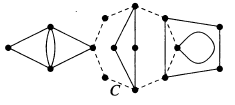
\includegraphics{img/ciclo-en-grafo-par.PNG}
            \caption{Podemos observar en este ejemplo que el grafo par efectivamente contiene un ciclo $C$.}
        \end{figure}
        
        \item[$\Rightarrow$] Supongamos que $G$ contiene un circuito euleriano $C$. Entonces cada vez que se enlista un vértice en $C$, deben haber dos lados incidentes en dicho vértice (uno de llegada y otro de salida). Por lo tanto todo vértice tiene grado par. Además, dos lados pueden estar en el mismo recorrido únicamente si están en la misma componente, por lo tanto $G$ tiene una sola componente no-trivial.
    \end{enumerate}
    
    Así queda demostrado.
\end{proof}

\begin{nota}
    En la demostración anterior utilizamos el siguiente hecho: Todo grafo par no trivial tiene un ciclo, y al eliminarlo, queda un grafo par. Así que por inducción obtenemos la siguiente proposición.
\end{nota}

\begin{pro}
    Todo grafo par se descompone en ciclos.
\end{pro}

Ahora, revisemos nuevamente el lema \ref{lem:2.3.1}. ¿Qué pasa si ahora agregamos la hipótesis de que el grafo $G$ es simple?

\begin{lem}
    Si $G$ es un grafo finito simple cuyos vértices tienen grado al menos $k$ entonces
    
    \begin{itemize}
        \item $G$ contiene un camino de longitud al menos $k$.
        \item Si además $k \geq 2$ entonces $G$ contiene un ciclo de longitud al menos $k+1$.
    \end{itemize}
\end{lem}

\begin{proof}
    Como es de esperar, utilizaremos un argumento análogo al del lema \ref{lem:2.3.1}.
    
    Como $G$ es finito, podemos considerar un camino maximal $P$ en $G$. Si $v$ es un extremo de $P$ entonces por maximalidad de $P$ y por hipótesis, $v$ tiene al menos $k$ vecinos en $P$. Por lo tanto la longitud de este camino es al menos $k$ y queda demostrada la primera parte.
    
    Consideremos ahora al vecino de $v$ más lejano (en el orden de la lista). Si $k \geq 2$ eso nos da para un ciclo en $G$ con longitud al menos $k+1$. Y así queda demostrado.
\end{proof}

\begin{pro}
    Todo grafo $G$ que tiene al menos un lado que no es un bucle, tiene al menos dos vértices que no son vértice-corte.
\end{pro}

\begin{proof}
    Si $u$ es un extremo de un camino maximal $P$ de $G$, entonces todos los vecinos de $u$ están en $P$. Como $P - u$ es conexo en $G - u$ concluímos que $v$ no es un vértice corte de $G$ y esto vale para ambos extremos de $P$.
    
    En total, tenemos al menos dos vértices que no son vértice corte y queda demostrado.
\end{proof}

\begin{lem}
    Si $G$ es un grafo par (finito), todo recorrido maximal en $G$ es cerrado.
\end{lem}

\begin{proof}
    Sea $R$ un recorrido maximal en $G$. Entonces cada paso de $R$ por un vértice $v$ usa dos lados incidentes en $v$ distintos. Al llegar a un vértice $v$ de $R$ distinto del inicial, $R$ ha usado una cantidad impar de lados incidentes con $v$. Como $v$ es par, $R$ debe continuar a otro vecino de $v$. Como $G$ es finito entonces $R$ debe continuar. Y como $G$ es par, debe terminar en el vértice inicial.
\end{proof}

\begin{prob}
    Al trazar una figura en papel, ¿cuántas veces como mínimo debemos detenernos y levantar el lápiz para continuar?. Si por ejemplo la figura es un circuito euleriano podemos hacerlo con un solo trazo, así que dependerá de cuántos vértices impares tenga el grafo correspondiente a la figura y la relación con la cantidad mínima de recorridos en que podemos descomponer el grafo.
    
    Supongamos por ahora que $G$ es conexo y tiene $2k$ vértices impares. Sabemos que un recorrido en el grafo contribuye a una cantidad par de lados en cada vértice interno y una cantidad impar en cada extremos (para un recorrido no cerrado). Por lo tanto, en toda partición en recorridos del conjunto de los lados, cada vértice impar es extremo de un recorrido no-cerrado. Como cada recorrido solamente tiene dos extremos, entonces debemos utilizar al menos $k$ recorridos para cubrir los $2k$ vértices impares del grafo $G$.
    
    Para $k = 0$ ya demostramos este problema en el teorema \ref{teo:suf-euler}. Nos queda demostrar únicamente cuando $k > 0$. Entonces pasemos a emparejar los vértices impares y agregamos un lado con cada par como extremos. El grafo resultante $H$ es conexo y par, así que tiene un circuito euleriano $C$. Al recorrer $C$, comenzamos un nuevo recorrido cada vez que pasamos por un lado de $H - E(G)$. Como agregamos $k$ lados, entonces tenemos a una descomposición de $G$ en $k$ recorridos.
\end{prob}

En síntesis, hemos demostrado el siguiente teorema:

\begin{teo}
    Si $G$ es un grafo finito, conexo y no-trivial, con $2k$ vértices impares, entonces $G$ se descompone como mínimo en $\max(1,k)$ recorridos.
\end{teo}

\begin{figure} % Otra vez. Flojera. Me quiero ir a acostar.
    \centering
    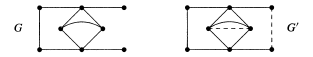
\includegraphics{img/descomposicion-recorridos.PNG}
    \caption{Ejemplo de la situación presentada en el problema anterior.}
\end{figure}